% Drawing 142/02-6 -- folder 142, batch 02, archive page 29 (PDF page 30).
% Transcription: sphère : pôles $P_{+}$ (en haut) et $P_{-}$ (en bas) ; sur l'équateur, les sommets $Q_0$, $Q_1$, $Q_\infty$ et les trois points marqués (ronds pleins) ; les arcs $\tilde a_i^{\pm}$ le long de l'équateur, et les méridiens $d_i^{+}$ (de $P_{+}$ à $Q_i$) et $d_i^{-}$ (de $P_{-}$ à $Q_i$), en trait plein ou en pointillé selon qu'ils sont vus ou cachés.
% Kind: sphere with poles, meridians and equatorial vertices. Method 2 (schematic redraw from the facsimile). Status: ok.
% Notes: Pencil outline; P^+ above, P_- below; on the equator Q_infty (back left), Q_0 (front), Q_1 (back right) and the three marked points (big dots: left edge, centre, right). Meridians: d_0^+ and d_0^- solid from the poles to Q_0 (arrows into Q_0); d_infty^+-, d_1^+- dashed from the poles to Q_infty and Q_1 (arrows into Q_infty and Q_1). Equatorial arcs, every one between the same vertex points: tilde a_1^+ and tilde a_1^- from Q_0 round the left edge to Q_infty (solid in front, dotted or dashed behind the edge), on either side of the left marked point; tilde a_0^+ and tilde a_0^- dashed between Q_infty and Q_1, on either side of the central point; tilde a_infty^+ and tilde a_infty^- from Q_0 round the right edge to Q_1, on either side of the right marked point. Labels as on the page; the label at the upper left reads tilde a_1^+ (the earlier redraw had tilde a_infty^+ there). Still differs: the label at the upper right edge reads like tilde a_0^+, but the arc it names joins Q_0 and Q_1, so it is set as tilde a_infty^+ (a reading); the sign of the lower middle label tilde a_0^- is hidden; the arrowheads on the equatorial arcs are a reading (into Q_0 for tilde a_1^- and tilde a_infty^+, into Q_1 for tilde a_0^+). The ink blot near Q_infty and the scribbled text above the sphere are not drawn. Nothing is struck. Redrawn 2026-11-09 (issue 128): to check again. 2026-11-13, Claude Opus 5.5, overlay check (issue 147): rasterised from its own coordinates over the 400 dpi colour scan (250 ppi native) on a unit grid, corrected, and laid over it again; not compiled (no TeX in the session). Changed: the outline was an ellipse 2 units above the page at the top and outside it at the upper right; it is traced as the freehand curve it is, through points read on the pencil (flattened at the top, where it runs into P^+), and the doubled pencil stroke at the lower right is drawn; the dashed meridians d_1^+ and d_1^- lay up to 3 units right of their dashes and are re-traced through them. The label at the upper right edge, read whole on the page beyond the edge of the crop, is tilde a_infty^+, as set (no longer a reading). Every stroke now lies on its ink to within about 1 unit. Kept as before: the sign of the lower middle label is hidden under the blot of the central marked point and is set tilde a_0^- (its pair above is tilde a_0^+); the heads are a reading of overinked strokes; the hatched blot above Q_infty (a crossing-out) and the writing above the sphere are not drawn.
% Coordinates: 1 unit = 1 mm = 1/100 of the crop width (bbox in page fractions: [0.12, 0.1, 0.37, 0.3]).
% Redrawn by Claude (claude-opus-5-5), issue #73, 2026-11-09; not checked by a human; not compiled (no TeX in the session).
% Checked by Claude (claude-opus-5-5) 2026-11-13 (issue #147): overlaid on the 400 dpi colour facsimile, corrected; not compiled (no TeX in the session). Not checked by a human. Status: ok.
% Rights: reproduces part of the work -- behind RENDER_TRANSCRIPTS, never published by itself.
\documentclass[tikz,border=3pt]{standalone}
\usepackage{amsmath,amssymb}
\usetikzlibrary{patterns,arrows.meta}
\tikzset{pencil/.style={black!45}, struck/.style={black!35}, mark/.style={circle,draw,inner sep=1.3pt}, pt/.style={circle,fill,inner sep=0.9pt}, opt/.style={circle,draw,fill=white,inner sep=1.1pt}}
\begin{document}
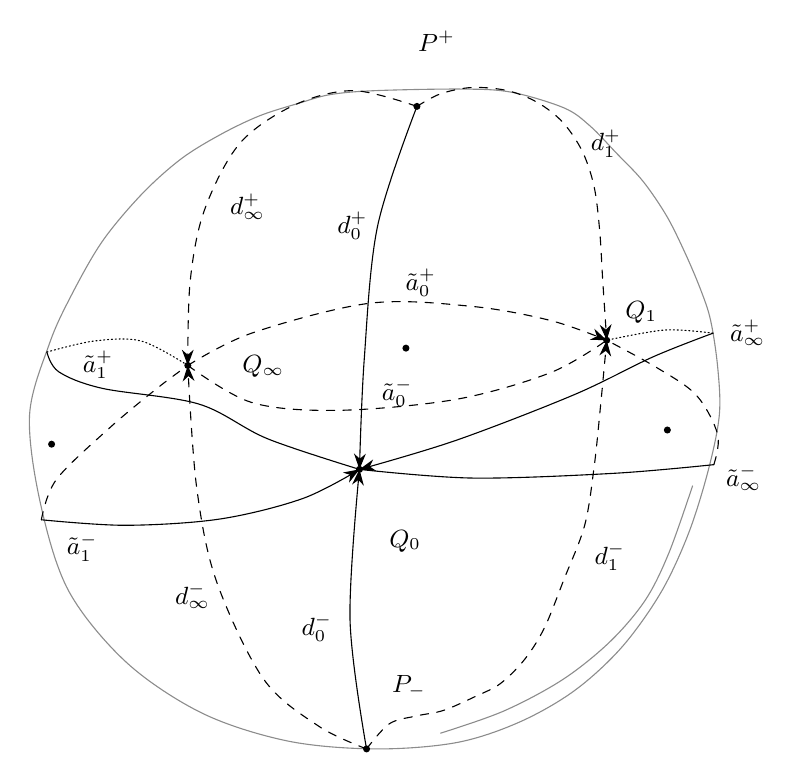
\begin{tikzpicture}[x=1mm,y=1mm,line cap=round,line join=round,font=\scriptsize]
\draw[pencil] plot[smooth cycle, tension=0.55] coordinates {(49.7,-27.8) (44,-28.3) (40,-29.4) (35,-31) (30,-33.4) (25,-36.5) (20,-41) (15,-47) (11,-54) (8.3,-60) (5.8,-69) (7.2,-80.3) (10.8,-91.4) (18.2,-100.5) (27.8,-106.9) (38.6,-110.4) (49.7,-111.4) (60,-110.6) (68,-108) (75,-104) (81,-98.5) (86,-91.5) (89.5,-84) (92,-76) (93.4,-69) (93.2,-63) (92.3,-57) (91,-53) (89,-48.3) (86.7,-43.7) (83.7,-39.3) (80.3,-35.7) (77,-32.3) (73.7,-30) (67,-28) (60.8,-27.6)};
\draw[pencil] plot[smooth, tension=0.55] coordinates {(90,-78) (87,-86.5) (84,-92.5) (79.5,-97.8) (73.5,-102.6) (66,-106.6) (58,-109.4)};
\node[pt] at (55,-29.8) {};
\node[pt] at (48.6,-111.4) {};
\node[pt] at (25.9,-62.7) {};
\node[pt] at (47.7,-75.9) {};
\node[pt] at (79.1,-59.5) {};
\node[pt] at (8.6,-72.7) {};
\node[pt] at (53.6,-60.5) {};
\node[pt] at (86.8,-70.9) {};
\draw[-{Stealth[length=2mm]}] plot[smooth, tension=0.55] coordinates {(55,-29.8) (50,-45) (48.3,-62) (47.7,-75.9)};
\draw[-{Stealth[length=2mm]}] plot[smooth, tension=0.55] coordinates {(48.6,-111.4) (46.5,-95) (47.7,-75.9)};
\draw[dashed,-{Stealth[length=2mm]}] plot[smooth, tension=0.55] coordinates {(55,-29.8) (47,-27.8) (39.5,-29.6) (32.5,-34.5) (28,-43) (26.2,-52) (25.9,-62.7)};
\draw[dashed,-{Stealth[length=2mm]}] plot[smooth, tension=0.55] coordinates {(48.6,-111.4) (42.5,-108.5) (35.5,-102.5) (29.5,-90) (27,-78) (25.9,-62.7)};
\draw[dashed,-{Stealth[length=2mm]}] plot[smooth, tension=0.55] coordinates {(55,-29.8) (58,-28.2) (62,-27.4) (66.5,-27.8) (70.3,-29.3) (73.5,-31.8) (76,-35.5) (77.5,-40) (78.2,-45.5) (78.6,-52) (79.1,-59.5)};
\draw[dashed,-{Stealth[length=2mm]}] plot[smooth, tension=0.55] coordinates {(48.6,-111.4) (51.5,-108.2) (55,-107.2) (58.4,-106.5) (62.5,-104.7) (65.6,-103.1) (68.7,-100) (71.2,-96) (73.7,-89.8) (76.3,-83) (77.5,-75.6) (78.3,-68) (79.1,-59.5)};
\draw plot[smooth, tension=0.55] coordinates {(47.7,-75.9) (36,-72) (27.3,-67.6) (15,-65.6) (9.5,-63.5) (8,-61)};
\draw[densely dotted] plot[smooth, tension=0.55] coordinates {(8,-61) (14,-59.6) (20,-59.6) (25.9,-62.7)};
\draw[-{Stealth[length=2mm]}] plot[smooth, tension=0.55] coordinates {(7.3,-82.3) (18,-83) (30,-82.2) (40.5,-79.6) (47.7,-75.9)};
\draw[dashed] plot[smooth, tension=0.55] coordinates {(7.3,-82.3) (9.2,-77.2) (16,-70.6) (22,-65.6) (25.9,-62.7)};
\draw[dashed,-{Stealth[length=2mm]}] plot[smooth, tension=0.55] coordinates {(25.9,-62.7) (34,-58.6) (49,-54.8) (62,-55.2) (72,-57) (79.1,-59.5)};
\draw[dashed] plot[smooth, tension=0.55] coordinates {(25.9,-62.7) (34,-67.4) (45,-68.4) (60,-67) (72,-63.6) (79.1,-59.5)};
\draw[-{Stealth[length=2mm]}] plot[smooth, tension=0.55] coordinates {(92.6,-58.6) (85,-61.6) (75,-66.4) (60,-72.2) (47.7,-75.9)};
\draw[densely dotted] plot[smooth, tension=0.55] coordinates {(92.6,-58.6) (86.5,-58.2) (79.1,-59.5)};
\draw plot[smooth, tension=0.55] coordinates {(47.7,-75.9) (62,-77) (80,-76.4) (92.7,-75.3)};
\draw[dashed] plot[smooth, tension=0.55] coordinates {(92.7,-75.3) (93.2,-71.5) (90.5,-66.5) (85.5,-63) (79.1,-59.5)};
\node[inner sep=1pt] at (57.5,-21.5) {\small $P^{+}$};
\node[inner sep=1pt] at (54,-103.5) {\small $P_{-}$};
\node[inner sep=1pt] at (35.5,-62.8) {\small $Q_\infty$};
\node[inner sep=1pt] at (53.5,-85) {\small $Q_0$};
\node[inner sep=1pt] at (83.5,-56) {\small $Q_1$};
\node[inner sep=1pt] at (33.5,-42.5) {\small $d_\infty^{+}$};
\node[inner sep=1pt] at (46.8,-45) {\small $d_0^{+}$};
\node[inner sep=1pt] at (79,-34.5) {\small $d_1^{+}$};
\node[inner sep=1pt] at (26.5,-92) {\small $d_\infty^{-}$};
\node[inner sep=1pt] at (42.3,-96) {\small $d_0^{-}$};
\node[inner sep=1pt] at (79.5,-87) {\small $d_1^{-}$};
\node[inner sep=1pt] at (14.5,-62.6) {\small $\tilde a_1^{+}$};
\node[inner sep=1pt] at (12.5,-85.8) {\small $\tilde a_1^{-}$};
\node[inner sep=1pt] at (55.5,-52.2) {\small $\tilde a_0^{+}$};
\node[inner sep=1pt] at (52.5,-66.2) {\small $\tilde a_0^{-}$};
\node[inner sep=1pt] at (97,-58.6) {\small $\tilde a_\infty^{+}$};
\node[inner sep=1pt] at (96.5,-77) {\small $\tilde a_\infty^{-}$};
\end{tikzpicture}
\end{document}
